\documentclass{article}
% these lines load any packages you might wish to use. 
% some common ones are loaded below
\usepackage{amsfonts, amsmath, amssymb}
\usepackage[numbers,square,sort&compress]{natbib}
\usepackage{graphicx}  % required for inserting images
\usepackage{hyperref}  % for inserting urls, and having clickable links to equation and figure numbers
\usepackage[margin=1.2 in]{geometry}  % these margins are easy to read
\geometry{letterpaper}                   % ... or a4paper or a5paper or ... 
\usepackage{lmodern}		% good font
\usepackage{appendix}
\usepackage{subcaption}
\usepackage{graphicx}

\usepackage{tikz}  % for using tikz, to draw your own figures
\usetikzlibrary{angles,quotes}

% input document information here
\title{Impact of Invasive Suckermouth Catfish on a Shrimp-Fish Predator-Prey System: A Lotka-Volterra Modeling Approach}
\author{Ryan Hsiao 61609715, Fanbo Feng 95719241, Davis Li 49877293}
%\date{}  % if you uncomment this, it will not put the date.
\date{Feb 6, 2026}   % if you uncomment this, it will list the date as whatever is inside the curly brackets


\begin{document}

\maketitle 

\section{Introduction} % Davis
There are many ecosystems that support the predator-prey model. Understanding how predation pressure interacts with natural recruitment is essential to explaining changes in prey populations and predicting the stability of nursery habitats. Studies have shown that some predators can consume multiple preys per day, while the prey rarely experience natural death when no predators are present [6][7]. In many regions, invasive species are reported to compete with native species, disrupting ecosystems [1][2][3]. These findings suggest that predator-prey interactions involving invasive species are a major determinant of prey populations.

\vspace{5mm}

\noindent We begin by modeling the system using the Lotka-Volterra equations. In the two-species predator-prey model based on experimental studies of shrimp and fish interactions [6][7], shrimp represent the prey population, while native fish represent the predator. We then introduce an invasive species named suckermouth catfish that competes for the same prey resource. Ecological studies show that loricariid catfish can produce dense populations and compete with native species for shared resources, potentially altering ecosystem dynamics [2][4]. From this point, we examine how the invasive species disrupts the steady state of the original two-species and alters long-term population dynamics. By analyzing the resulting three-species system, we aim to determine the new steady states and identify conditions for coexistence or population decline.

\subsection*{Problem Statement}
We investigate how an invasive fish species affects an established predator-prey system consisting of native shrimp (prey) and predatory fish. Starting from a two-species steady state of the native system, we then address the following questions:
\begin{itemize}
\item \textbf{How does the introduction of invasive suckermouth fish that consume the same prey as native predators disrupt the original equilibrium?}
\item \textbf{Can a simple Lotka-Volterra-type predator-prey model predict the new long-term steady state or dynamics including potential outcomes such as coexistence of all three species, exclusion of native prey, or displacement of native predator?}
\end{itemize}

\vspace{5mm}

\noindent Combining ecological reasoning with mathematical analysis, we aim to explore whether the key features of predator-prey dynamics can be captured with a simple model. The results help clarify the sensitivity of coastal shrimp populations to changes in predation and recruitment, and highlight both the strengths and limitations of using classical predator-prey models for real-world ecosystems.


\section{Building the three-species model}\label{sec:model} 
%% Most general and original model for preditor prey system. 
%% Explain it.
\subsection{Definitions and notation} % Ryan

%%%%%%%%%%%%%%%%%%%%%%%%%%%%%%%%%%%%%%%%%% Table start
\begin{table}[!h]
\begin{center}
\begin{tabular}{||c | c | c||} 
 \hline
 Symbol & Description & Dimensions \\ [0.5ex] 
 \hline\hline
 $x$ & The population of species X (prey). & N \\ 
 \hline
 $y$ &  The population of species Y (predator).  & N \\ 
 \hline
 $z$ & The population of species Z (invasive species).  & N \\ 
 \hline
 $x_0$ &  The initial population of species X (prey). & N \\ 
 \hline
 $y_0$ & The initial population of species Y (predator).  & N \\ 
 \hline
 $z_0$ & The initial population of invasive species Z (invasive species).  & N \\ 
 \hline
 $t$ & Time.  & T \\ 
 \hline
 $\alpha$ & The growth rate of prey (X) in the absence of a predator (Y).  & T$^{-1}$ \\ 
 \hline
 $\beta$ & The death rate of prey (X) due to the predation.  & T$^{-1}$N$^{-1}$ \\
 \hline
 $\varepsilon$ & The death rate of prey (X) due to food sharing with invasive species. & T$^{-1}$N$^{-1}$ \\
 \hline
 $\gamma$ & The natural death rate of predator (Y).  & T$^{-1}$ \\
 \hline
 $\delta$ & The growth rate of the predator (Y) due to predation on the prey.   & T$^{-1}$N$^{-1}$ \\
 \hline
 $\xi$ & The growth rate of invasive species (Z). & T$^{-1}$ \\
 \hline
 $\sigma$ & The death rate of invasive species (Z) due to food sharing with prey. & T$^{-1}$N$^{-1}$ \\ [1ex] 
 \hline
\end{tabular} 
\end{center}
\captionsetup{font=small}
\caption{The variables and parameters are measured in year (dimension T) and million individuals (dimension N).} % All dimensions N has the unit of million, and dimensions of T has the unit of year.
\end{table}
%%%%%%%%%%%%%%%%%%%%%%%%%%%%%%%%%%%%%%%%%% Table end

\noindent There are many ecosystems consisting of three species. Our objective is to determine the type of ecosystem as follows: the ecosystem we study involves a three species food chain system where prey ($x$) and invasive species ($z$) are at the lowest level of the food chain such that they do not consume each other, and the predator ($y$) is at the highest level. In addition, invasive species do not have a predator---the existing predator does not consume the invasive species, as stated in the introduction.

\vspace{5mm}

\noindent Next, we assume conditions to simplify the model from the real word scenario in order to achieve the target model mentioned above. First, the death of the prey will be due to predation and food sharing with the invasive species. Furthermore, the death of the predator will only be caused by natural death as it does not have a higher degree predator present in the system, and the growth rate will only be due to predation on the prey. Finally, the death of the invasive species will be due to food sharing with the prey presented in the system. In addition, all parameters in Table 1 are constant and do not change over time, and food for prey and invasive species is limited. The lack of food will cause changes in the population. These conditions are assumed to give limitations to each species so that their population changes based on birth, predation, and starvation, which are essential elements of an ecosystem.

\vspace{5mm}

\noindent Finally, since we consider a realistic ecosystem, we have constrained our variables and parameters as follows: $x\ , y \ , z \ , x_0 \ , y_0 \ , z_0 \ge 0$, $t\ge0$, and $\alpha \ , \beta \ , \varepsilon \ , \gamma \ , \delta \ , \xi \ , \sigma \ge0$. In addition, the population is measured in \textit{millions of individuals} and \textit{year} for time, similarly for the rate parameters (Table 1).

\subsection{Classical two species Lotka-Volterra equations}
\noindent The general Lotka-Volterra equation existed in the literature consists of a prey and a predator that shows the change in the population of prey ($x$) and predator ($y$). It accounts for the growth rate ($\alpha$) and the death rate ($\beta$) with and without the predator for prey and the natural death rate ($\gamma$) and the growth rate ($\delta$) due to predation by the predator. 

\vspace{5mm}

\noindent The model was introduced in the 1920s by Vito Volterra, who wished to use this model to observe the population change of predator fish in the Adriatic Sea during WWI [8]. This model is very similar to the three-species model that we aim to study in this paper. 

\noindent The Lotka-Volterra equation is shown as follows:

\begin{align*}
    \begin{cases}
        \dfrac{dx}{dt} = \alpha x - \beta x y \ , \\
        \\
        \dfrac{dy}{dt} = -\gamma y + \delta x y \ ,
    \end{cases}   \tag{2.1}
\end{align*}

\noindent where the notations of variables and parameters are shown in Table 1.

\subsection{Introducing the third-species into the Lotka-Volterra equations}
\noindent Introducing an invasive species into the system gives a new term in the ODE describing prey and a new ODE describing invasive species based on our assumption above. 

\vspace{5mm}

\noindent First, we look at the differential equation for the prey ($x$), there will be an additional term $\varepsilon xz$, which describes population loss due to food sharing with invasive species ($z$). This term shares a similar idea to $\beta xy$ that the prey is competing with the predator. 

\vspace{5mm}

\noindent Next, we look at the new equation for the invasive species ($z$), the equation shares a similar idea to the prey that the change in population is described by the population growth term $\xi z$ subtracting the population loss due to competition ($\sigma xz)$ with the prey. The equation do not have a third term as it do not eat by other species presented in the ecosystem, i.e., there is no predator for invasive species.

\vspace{5mm}

\noindent Combining the two-species ecosystem (2.1) mentioned above with the new terms described, the three-species ecosystem with an invasive species can be modeled as follows:

\begin{align*}
    \begin{cases}
        \dfrac{dx}{dt} = \alpha x - \beta x y - \varepsilon x z\ ,  \\
        \\
        \dfrac{dy}{dt} = -\gamma y + \delta x y \ , \\
        \\
        \dfrac{dz}{dt} = \xi z - \sigma x z \ ,
    \end{cases} \tag{2.2}
\end{align*}

\noindent and 

\begin{align*}
    x(0) = x_0 \ , \hspace{0.5in} y(0) = y_0 \ , \hspace{0.5in} z(0) = z_0 \ ,  \tag{2.3}
\end{align*}

\noindent where the descriptions and representations of the symbols in (2.2) are shown in Table 1 and (2.3) represents the initial conditions of the three species' population. 

\subsection{Nondimensionalization} % Ryan
The variables and parameters used in the system of equations (2.2) have base quantities and dimensions, which we can non-dimensionalize. 

\vspace{5mm}

\noindent By performing the nondimensionalization process, we get the following system of equations:

\begin{align*}
    \begin{cases}
        \dfrac{dx^*}{dt^*} = x^* - x^*y^* - x^*z^* \ , \\
        \\
        \dfrac{dy^*}{dt^*} = a(-y^* + x^*y^*) \ , \\
        \\
        \dfrac{dz^*}{dt^*} = bz^* - cx^*z^* \ ,
    \end{cases} \tag{2.4} 
\end{align*}

\noindent and 

\begin{align*}
    x^*(0) = dx_0 \ , \hspace{0.5in} y^*(0) = ey_0 \ , \hspace{0.5in} z^*(0) = fz_0 \ , \tag{2.5}
\end{align*}

\noindent where $a = \dfrac{\gamma}{\alpha}$, $b = \dfrac{\xi}{\alpha}$, $c = \dfrac{\sigma \gamma}{\alpha\delta}$, $d = \dfrac{\delta}{\gamma}$, $e = \dfrac{\beta}{\alpha}$, and $f = \dfrac{\varepsilon}{\alpha}$. 

\vspace{5mm}

\noindent The process of nondimensionalization can be checked in Appendix A. After scaling (2.2), we get (2.4) as the result and all variables $x^*$, $y^*$, $z^*$, and $t^*$ are now dimensionless.

\section{Analysis of the three-species Lotka-Volterra equations}

\subsection{Computing the steady-states} % Fanbo
The steady-state occurs when:
$$
\begin{aligned}
\alpha x - \beta xy - \varepsilon xz &= 0 \ ,\\
-\gamma y + \delta xy &= 0 \ ,\\
\xi z - \sigma xz &= 0 \ .
\end{aligned}
$$

\noindent The first equation gives us $x = 0$ and $\beta y + \varepsilon z = \alpha$. The second equations have solutions $y=0$ and $x = \frac{\gamma}{\delta}$. The third equations have solutions $z = 0$ and $x = \frac{\xi}{\sigma}$.

\vspace{5mm}

\noindent We can first generate a steady-state with $(x,y,z) = (0, 0, 0)$. For $x \ne 0$, we have two choices with $x = \frac{\gamma}{\delta}$ and $x = \frac{\xi}{\sigma}$. With these choices of the $x$ value, we also have the relation between $y$ and $z$ that satisfies the equation : $\beta y + \varepsilon z = \alpha$, i.e. $y = \frac{\alpha}{\beta} - \frac{\xi}{\beta}z$. If $y \ne 0$, then we must let $x = \frac{\gamma}{\delta}$ to make the left hand side of the second equation equal to zero, so we can obtain $z = 0$  and $y = \frac{\alpha}{\beta}$. Similarly, if $z \ne 0$, we must have $y=0$ with $x = \frac{\xi}{\sigma}$, $z = \frac{\alpha}{\xi}$ to satisfy all equations. Therefore, we have 3 steady-states for this system of equations:

$$
(x,y,z) = (0, 0, 0), \qquad (x,y,z) = (\frac{\gamma}{\delta}, \frac{\alpha}{\beta}, 0), \qquad (x,y,z) = (\frac{\xi}{\sigma}, 0, \frac{\alpha}{\xi}).
$$

\vspace{3mm}

\noindent For the first steady-state, it shows that our system is stable when all species have 0 population, signifying the extinction of three species. For the second and third steady-states, they both contain a 0 in their values, i.e., the 0 population in invasive species and predator respectively. This means the system will reach a stable state only if the population of either invasive species or predator becomes 0.

\subsection{Checking the stability}
\noindent Subsequently, we define a vector function $F(x,y,z)$ which contains three scalar functions $f(x,y,z)$, $g(x,y,z)$, and $h(x,y,z)$:
$$
F(x,y,z) 
= \begin{pmatrix}
f(x,y,z)\\
g(x,y,z)\\
h(x,y,z)
\end{pmatrix} 
= \begin{pmatrix}
\alpha x - \beta xy - \varepsilon xz \\
-\gamma y + \delta xy\\
\xi z - \sigma xz
\end{pmatrix} \ .
$$

\noindent We then write a Jacobian matrix with functions $f$, $g$, $h$:
$$
J = 
\begin{pmatrix}
f_x & f_y & f_z\\
g_x & g_y & g_z\\
h_x & h_y & h_z
\end{pmatrix} 
= \begin{pmatrix}
\alpha - \beta y - \varepsilon z & -\beta x & \varepsilon x \\
\delta y & -\gamma + \delta x  & 0\\
- \sigma z & 0 & \xi - \gamma x
\end{pmatrix} \ .
$$
\noindent Thus, we can apply our three steady-state points on this Jacobian to analyze the stability of each point.

\subsubsection*{Apply the steady-state $\bf (x_1,y_1,z_1) = (0, 0, 0)$}
we get:
\begin{align}
J
= \begin{pmatrix}
\alpha - \beta y - \varepsilon z & -\beta x & \varepsilon x \\
\delta y & -\gamma + \delta x  & 0\\
- \sigma z & 0 & \xi - \gamma x
\end{pmatrix}\Big|_{(x_1, y_1,z_1)}
= \begin{pmatrix}
\alpha & 0 & 0 \\
0 & -\gamma & 0\\
0 & 0 & \xi
\end{pmatrix} \ .
\tag{3.1}
\end{align}

\noindent By calculating the determinate of this matrix, we obtain the eigenvalues:
$$\lambda_1 = \alpha, \qquad \lambda_2 = -\gamma, \qquad \lambda_3 = \xi.$$

\noindent Since we have two positive eigenvalues, this steady-state is an unstable saddle. In the aspect of our system, this reflects that both prey and invasive species have positive intrinsic growth rates, so any small introduction of these species will cause the system to move away from extinction. Therefore, complete extinction is not a sustainable equilibrium in this model.


\subsubsection*{Apply the steady-state $\bf(x_2,y_2,z_2) = (\dfrac{\gamma}{\delta}, \dfrac{\alpha}{\beta}, 0)$}
\begin{align}
J = \begin{pmatrix}
\alpha - \beta y - \varepsilon z & -\beta x & \varepsilon x \\
\delta y & -\gamma + \delta x  & 0\\
- \sigma z & 0 & \xi - \gamma x
\end{pmatrix}\Big|_{(x_2,y_2,z_2)}
= \begin{pmatrix}
0 & -\frac{\beta \gamma}{\delta} & -\frac{\varepsilon \gamma}{\delta} \\
\frac{\delta \alpha}{\beta} & 0 & 0\\
0 & 0 & \xi - \frac{\sigma \gamma}{\delta}
\end{pmatrix} \ .
\tag{3.2}
\end{align}

\noindent Using the same calculation method above, we have the eigenvalues: 
$$\lambda_{1,2} = \pm i \sqrt{\alpha \gamma}\ , \qquad \lambda_3 = \xi - \frac{\sigma \gamma}{\delta} \ .$$

\noindent Since we have two pure imaginary eigenvalues here, we see that the solution spirals around this steady-state, and so we have the third eigenvalue $\lambda_3 = \xi - \frac{\sigma \gamma}{\delta}$ which determines the stability. If $\lambda_3 > 0$, it is unstable; if $\lambda_3 < 0$, it is a stable spiral. For the special case $\lambda_3 = 0$, we have $\xi - \frac{\sigma \gamma}{\delta} = 0$, i.e., $\frac{\gamma}{\delta} = \frac{\xi}{\sigma} = x$. Thus, we cannot compute this clear steady-state $(x_2,y_2,z_2)$ because $y$ and $z$ can be both non-zero in these special cases, which make the three equations we get in (3.1) unsolvable, so we do not discuss this case here. Next, in biological meaning, if $\lambda_3 < 0$, invasive species cannot grow when rare and the native ecosystem is resistant to invasion; if $\lambda_3 > 0$, invasive species can increase from small population levels, destabilizing the native equilibrium. Thus, this condition provides a mathematical threshold for successful invasion.

\subsubsection*{Apply the steady-state $\bf(x_3,y_3,z_3) = (\dfrac{\xi}{\sigma}, 0, \dfrac{\alpha}{\xi})$}

\begin{align}
J = \begin{pmatrix}
\alpha - \beta y - \varepsilon z & -\beta x & \varepsilon x \\
\delta y & -\gamma + \delta x  & 0\\
- \sigma z & 0 & \xi - \gamma x
\end{pmatrix}\Big|_{(x_3, y_3,z_3)}
= \begin{pmatrix}
0 & -\frac{\beta \xi}{\sigma} & -\frac{\varepsilon \xi}{\sigma} \\
0 & -\gamma + \frac{\delta \xi}{\sigma} & 0\\
-\frac{\sigma \alpha}{\varepsilon} & 0 & 0
\end{pmatrix} \ .
\tag{3.3}
\end{align}

\noindent By the same calculation method, the eigenvalues are:
$$\lambda_{1,3} = \pm \sqrt{\alpha \xi}\ ,  \qquad \lambda_2 = \gamma - \frac{\delta \xi}{\sigma} \ .$$

\noindent Since we have a positive sign from $\lambda_{1,3}$, this steady point is always unstable. By calculating its determinant, we get $\frac{\alpha \xi (\gamma \sigma - \xi \delta)}{\sigma}$. If $\gamma \sigma - \xi \delta < 0$, the steady-state is an unstable saddle; otherwise, it is not a saddle but is still unstable. Additionally, if we let the determinant equal to 0, we get the same situation as in the special case in our $(x_2,y_2,z_2)$ steady-state, which is a contradiction for the third steady-state. Therefore, this steady-state is always unstable, and small perturbations will drive the system away from this equilibrium, implying that stable long-term coexistence of only prey and invasive species is not possible in our model. 

\section{Results of the population change between the three-species} % Ryan
%% Inteprating the model with specific species

\begin{figure}[htbp]
     \centering
     \begin{subfigure}[b]{0.3\textwidth}
         \centering
         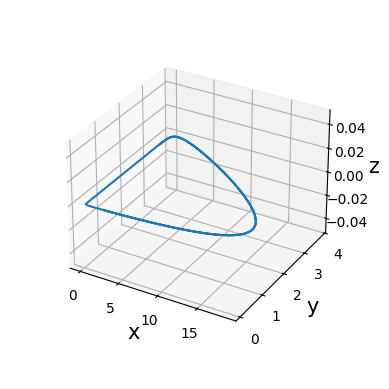
\includegraphics[width=\textwidth]{data/1a.png}
         \caption{$z=0$}
     \end{subfigure}
     \hfill
     \begin{subfigure}[b]{0.3\textwidth}
         \centering
         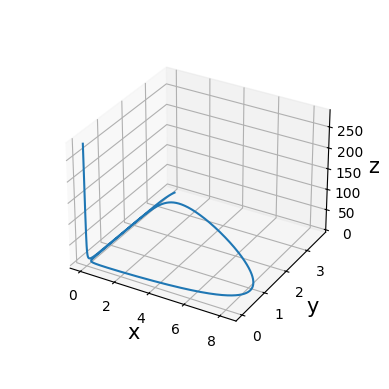
\includegraphics[width=\textwidth]{data/1b.png}
         \caption{$x,y,z\not=0$}
     \end{subfigure}
     \hfill
     \begin{subfigure}[b]{0.3\textwidth}
         \centering
         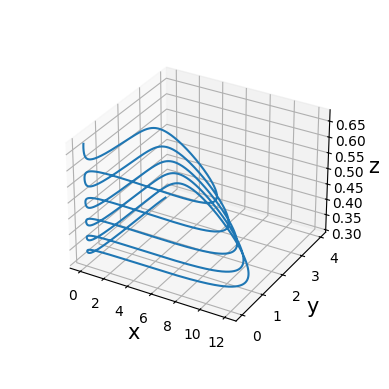
\includegraphics[width=\textwidth]{data/1c.png}
         \caption{Real data}
     \end{subfigure}
     \captionsetup{font=small}
     \caption{In this figure, we have the x-axis representing the prey, y-axis representing the predator, and the z-axis representing the invasive species. This set of plots shows the change in population of the three-species.}
\end{figure}

\begin{figure}[htbp]
     \centering
     % Second Row
     \begin{subfigure}[b]{0.3\textwidth}
         \centering
         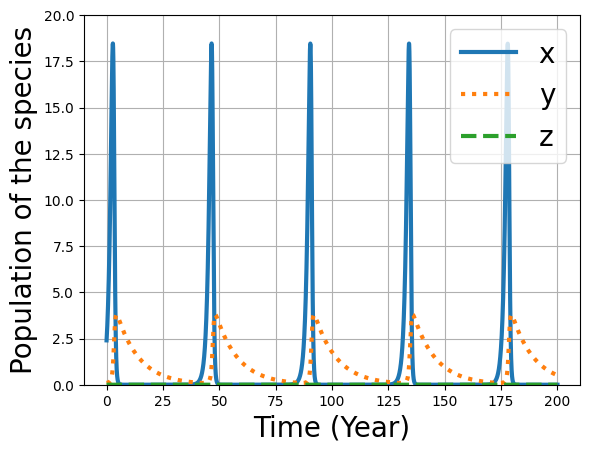
\includegraphics[width=\textwidth]{data/2a.png}
         \caption{$z=0$}
     \end{subfigure}
     \hfill
     \begin{subfigure}[b]{0.3\textwidth}
         \centering
         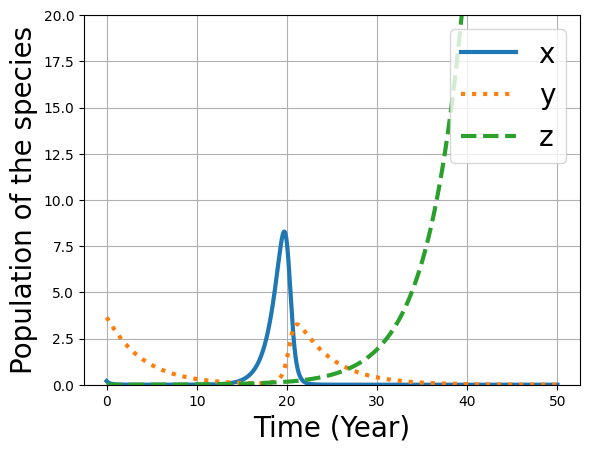
\includegraphics[width=\textwidth]{data/2b.png}
         \caption{$x, y, z \not=0$}
         \label{fig:exp x}
     \end{subfigure}
     \hfill
     \begin{subfigure}[b]{0.3\textwidth}
         \centering
         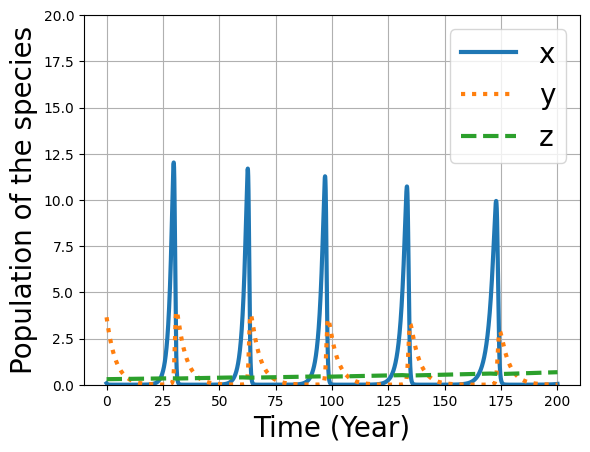
\includegraphics[width=\textwidth]{data/2c.png}
         \caption{Real data}
     \end{subfigure}
     \captionsetup{font=small}
     \caption{In this figure, we have the horizontal x-axis representing the time (year) and the vertical y-axis representing the number of populations of the three-species. The plots shows the change of population between three-species separately.}
\end{figure}

\noindent Based on experimental feeding rates [6], fish consumed approximately 2-13 juvenile shrimp per day at moderate prey densities, so we picked a middle value and set $\beta = 73$. The intrinsic growth rate of shrimp $\alpha = 4$ was estimated from the observed juvenile turnover in estuarine habitat research [6][7], corresponding to population dynamics on an annual timescale. The predator mortality parameter $\gamma$ was calibrated using the characteristic prey density scale observed in predator-prey experiments [6][7]. Using the break-even condition $\gamma = \delta x^*$, where $x^*$ represents a typical shrimp population density [6][7], we chose $\gamma = 1$ to ensure ecological consistency between prey availability and predator persistence. The conversion parameter $\delta$ represents the fraction of consumed prey that is converted into predator growth. Since only shrimp consumption is measured but not predator growth per prey eaten [6][7], we cannot directly obtain $\delta$ from the experimental data. Instead, $\delta$ was treated as an effective ecological parameter and selected to balance predator growth with the calibrated mortality rate $\gamma$, ensuring realistic population dynamics. This ensures that the predator population does not change unrealistically. The parameters $\varepsilon$, $\xi$, $\sigma$ are all related to invasive species such that $\varepsilon$ and $\sigma$ are related to competition due to food sharing, which is difficult to quantify and find the value to best describe it. Hence, we choose $\varepsilon = 0.2$ and $\sigma = 0.1$ as they should be smaller than or close to the natural death rate of the sucker-mouth fish [3]. Based on reasonability, death from food sharing should be lower compared to death from predation ($\beta$). Then, we get the parameter $\xi = 0.025$ based on the research paper on the life cycle of the sucker-mouth fish [1].
% The data implemented in Figure 1(c) and Figure 2(c).

\vspace{5mm}

\noindent We can compute three different results for the relation and population change of three species by choosing different combinations of parameters values. Since the values of parameters we get based on the research have a large scale which is hard to observe wether the result reaches steady-state, for Figure 1(a) and Figure 2(a), we choose the initial conditions, $x_0=0.8$, $y_0 = 0.2$, $z_0 = 0$, for the two-species stable-state. The parameters are set to $\alpha = 1$, $\beta = 0.5$, $\varepsilon = 0.2$, $\gamma = 1$, $\delta = 0.1$, $\xi = 0.025$, and $\sigma=0.1$, for a better visualization on steady-state. Furthermore, for Figure 1(b) and Figure 2(b), the initial conditions are set to $x_0=0.8$, $y_0 = 0.2$ and $z_0 = 0.1$ since we introduce the invasive species. The parameters are set to $\alpha = 4$, $\beta = 73$, $\varepsilon = 0.05$, $\gamma = 1$, $\delta = 0.25$, $\xi = 1$, and $\sigma=0.125$ so that we can have a better observation on the impact made by the invasive species. In Figure 1(c) and Figure 2(c), we define $\alpha = 4$, $\beta = 73$, $\varepsilon = 0.2$, $\gamma = 1$, $\delta = 0.1$, $\xi = 0.025$, and $\sigma = 0.1$, which are the data we obtained from the research, and tune our initial conditions based on them. After testing, we pick $x_0 = 0.8$, $y_0 = 0.2$, and $z_0 = 6$ for clearer illustration.

\subsection*{Implementation and numerical methods}

\noindent The plots shown in Figures 1 and 2 are generated by Python with Scipy and Matplotlib. We first initialize initial conditions such as $x_0$, $y_0$, $z_0$, and other parameters in Table 1. Next, we can create a Python method that takes in a vector form of the rewritten form of system (2.4) with new variables, $u_0 = x$, $u_1 = y$, and $u_2 = z$, as input, and returns a vector of $\dfrac{du}{dt}$. Then, we plug the method we defined with the initial condition of $u_0 = [x_0^*, y_0^*, z_0^*]$ into the Scipy method Odeint for the result, where Odeint solves for the system of differential equations. Finally, with the output generated by Odeint, we are able to plot the results shown in Figures 1 and 2. Check the Github repository for more detailed implementation.

\section{Discussion}

\subsection*{Two-species stable-state}

\noindent We aim to analyze the impact of an invasive species on a natural ecosystem containing two species and whether the system is in a steady state. This is shown in Figures 1(a) and Figure 2(a) setting the $z$ variable in equation (2.2) to 0 to remove it from the system for now.

\vspace{5mm}

\noindent From the stability analysis section above, the analysis for matrix (3.2) tells us that there exists a steady-state, and the solution is spiral around the steady-state since the eigenvalues are imaginary and $\lambda_3 = \xi - \frac{\sigma\gamma}{\delta}=0.025-\frac{0.1\cdot1}{0.1}\approx -0.975 <0$. This result is identical to what is shown in Figure 1(a) and Figure 2(a). As shown in both plots, the population of the prey increases when the population of the predator is low and decreases as the population of the predator increases; similarly for the predator. Hence, they reach a dynamic equilibrium state over time.

\subsection*{Introducing the invasive species}

\noindent Now, from the above section, we have a steady ecosystem consisting of two species, then we introduce a new invasive species into the system of equations, which is indicated in equation (2.2). The stability analysis above reveals that the steady-state is unstable by the determinant of matrix (3.3) such that $\gamma\sigma - \xi\delta = 1\cdot 1 - 1\cdot \frac{1}{4}\ge0$ with one of the eigenvalues always negative and one positive. On the other hand, with matrix (3.1), we can conclude that the three-species system has a steady-state of unstable saddle. This is similar to what we observed in Figure 1(b). In Figure 2(b), we observe that the relations between the prey and predator populations seem like a steady-state while the population of invasive species is low. However, as the population of the invasive species increases over time, the populations of the other two species approach zero. This results in a system of the invasive species dominating the system with exponential growth, i.e., eliminating all other species. 

\subsection*{Analyze with real world data}

\noindent Lastly, as the plots above match our expectations based on the stability analysis, we can implement more realistic data such as sucker-mouth fish introduced to a stable ecosystem of fish and shrimp. For a small initial sucker-mouth fish population such as $z_0=0.8$ and $z_0=0.2$, the population growth of it will be very slow, so it would take hundreds of years to have a significant impact on the system. However, with an initial population set to six million individuals, we observed a slight increase in the suck-mouth fish population approximately 200 years after the introduction. On the other hand, we observed that the peak populations of prey and predators are decreasing over time in Figure 2(c). More importantly, we observed a more obvious spiral solution for the three-species system describing the correlation between them, which is expected from the stability analysis in Figure 1(c).

\vspace{5mm}

\noindent With different values of parameters, we observed that the destruction of the ecosystem due to invasive species is highly dependent on parameters $\xi$ and $\sigma$ such that it will affect the speed of deconstruction of the original system, i.e., the breed of invasive species. At the same time, increasing the initial population of invasive species ($z_0$) does not change much. 

\section{Conclusion} % Davis
This project has investigated how an invasive suckermouth armored catfish impacted a native estuarine predator-prey system that involved brown shrimp and established predatory fish. Starting from a two-species steady state, we extended the classic Lotka-Volterra process to a three-species model and examined the resulting long-term dynamics through stability analysis and numerical simulations.

\vspace{5mm}

\noindent The results show that the invasive species disrupt the original steady state, often leading to oscillatory spirals around the native equilibrium followed by gradual decline of both prey and native predator populations. When the invasive growth rate ($\xi$) or the intensity of competition ($\sigma$) reaches a certain level, the system tilts in favor of the invasive species, with populations of native shrimp and predatory fish approaching zero. These results highlight the sensitivity of coastal nursery habitats to additional resource competitors and highlight how even modest invasive populations can cause long-term ecological shifts over hundreds of years.

\vspace{5mm}

\noindent Although classic predator-prey models are easy to interpret and can capture key behaviors such as population oscillations and competitive exclusion, they have limitations in real estuarine ecosystems. Our model relies on several simplifying assumptions: predation follows a linear functional response, shrimp and invasive fish grow without density dependence, and populations are well mixed without spatial structure. We also assume the invasive catfish to feed only on shrimp without alternative food sources or non-consumptive effects such as behavioral avoidance. The model also omits key features of real shrimp nurseries, including seasonal recruitment, vegetation refuges, habitat modification by suckermouth fish, and environmental variability.

\vspace{5mm}

\noindent Our model could be extended along several lines. Introducing logistic growth for shrimp would make prey dynamics more realistic. Incorporating spatial processes, such as refuge zones, and accounting for habitat modification by invasive species would better reflect field conditions. Parameter estimation from real time-series data in invaded regions, along with broader sensitivity analysis, would improve the model’s ability to make quantitative predictions. In addition, modeling intraguild predation between native predators and invasive species could reveal more complex coexistence outcomes.

\vspace{5mm}

\noindent Overall, this project demonstrates that the introduction of a shared-resource competitor can fundamentally reshape predator-prey equilibria in coastal ecosystems. Simple models like ours provide a useful entry for understanding invasion dynamics and guiding efforts to conserve shrimp populations. This project deepened our understanding of how invasive species can alter predator–prey dynamics: not only through direct consumption, but also through competition for shared resources. We observed how coexistence outcomes depend on relative growth and mortality rates and how even minor changes in parameter values can shift the system between stability and instability. 


%%%%%%%%%%%%%%%%%%%% Refrence Start %%%%%%%%%%%%%%%%%%%%%%%%%%%
\bibliographystyle{plain} % you can choose from many different styles: https://www.overleaf.com/learn/latex/Bibtex_bibliography_styles
\begin{thebibliography}{7} % Entries are in the Refs.bib file
\bibitem[1]{one}
Silvana Duarte, Francisco Gerson Araújo, and Nilo Bazzoli. 
Reproductive plasticity of Hypostomus affinis (Siluriformes: Loricariidae) as a mechanism to adapt to a reservoir with poor habitat complexity. \emph{Zoologia}, 28(5):577-586, 2011.
\bibitem[2]{two}
S. Luci Cook-Hildreth, Timothy H. Bonner, and David G. Huffman. Female reproductive biology of an exotic suckermouth armored catfish (Loricariidae) in the San Marcos River, Hays Co., Texas, with observations on environmental triggers. \emph{BioInvasions Records}, 5(3):173-183, 2016.
\bibitem[3]{three}
Md. Taskin Parvez, Martyn C. Lucas, Md. Ishrak Hossain, Nipa Chaki, A. B. M. Mohsin, Jingrui Sun, and Shams M. Galib. Invasive vermiculated sailfin catfish (Pterygoplichthys disjunctivus) has an impact on highly valued native fish species. \emph{Biological Invasions}, 25:1795-1809, 2023.
\bibitem[4]{four}
Thanapop Sotehome (or Sotehome) and Sumapa Thedkwanchai. Product Development of Fish Crisp from Sucker Mouth Fish (Hypostomus plecostomus). \emph{Journal of Advanced Zoology}, 44:1311-1321, 2023.
\bibitem[5]{five}
Katrina L. Pound, Weston H. Nowlin, David G. Huffman, and Timothy H. Bonner. Trophic ecology of a nonnative population of suckermouth catfish (Hypostomus plecostomus) in a central Texas spring-fed stream. \emph{Environmental Biology of Fishes}, 90:277-285, 2011.
\bibitem[6]{six}
Thomas J. Minello and Roger J. Zimmerman. Fish predation on juvenile brown shrimp, Penaeus aztecus Ives: the effect of simulated Spartina structure on predation rates. \emph{Journal of Experimental Marine Biology and Ecology}, 72:211-231, 1983.
\bibitem[7]{seven}
Thomas J. Minello, Roger J. Zimmerman, and Eduardo X. Martinez. Fish predation on juvenile brown shrimp, Penaeus aztecus Ives: effects of turbidity and substratum on predation rates. \emph{Fishery Bulletin}, 85(1):59-70, 1987.
\bibitem[8]{eight}
Chauvet, E., Paullet, J. E., Previte, J. P., Walls, Z. (2002). A Lotka-Volterra Three-Species Food Chain. \emph{Mathematics Magazine}, 75(4), 243–255.

\end{thebibliography}
%%%%%%%%%%%%%%%%%%%% Reference end %%%%%%%%%%%%%%%%%%%%%%%%%%%%%

%%%%%%%%%%%%%%%%%%%% Appendix Start %%%%%%%%%%%%%%%%%%%%%%%%%%%%%
\appendix
\section*{Appendix A}
Population $x$, $y$, and $z$ are dependent variables; time $t$ is the independent variable. Then, let $t = [t]t^*$, $x = [x]x^*$, $y = [y]y^*$, $z = [z]z^*$, and substitute these into the system of equations (2.2). Next, We choose:
$$
[x] = \frac{\gamma}{\delta}, \quad [y]= \frac{\alpha}{\beta}, \quad[z] = \frac{\alpha}{\varepsilon} \ .
$$
Since we cannot choose a $[t]$ such that all coefficients are 1, we choose from:
$$
[t] = \frac{1}{\alpha}, \quad [t] = \frac{1}{\gamma}, \quad [t] = \frac{\delta}{\sigma \gamma} \ .
$$

\noindent Let $[t] = \frac{1}{\alpha}$. We rewrite the equations:

$$
\begin{aligned}
\frac{dx^*}{dt^*} &= x^* - x^*y^* - x^*z^* \ , \\
\frac{dy^*}{dt^*} &= a(-y^* + x^*y^*) \ , \\
\frac{dz^*}{dt^*} &= bz^* - cx^*z^* \ ,
\end{aligned}
$$

$$
x^*(0) = dx_0, \quad y^*(0) = ey_0, \quad z^*(0) = fz_0 \ .
$$

\noindent where:
$$
a = \frac{\gamma}{\alpha},\quad b = \frac{\xi}{\alpha}, \quad c = \frac{\sigma \gamma}{\alpha \delta},  \quad d = \frac{\delta}{\gamma}, \quad e = \frac{\beta}{\alpha},  \quad f = \frac{\varepsilon}{\alpha} \ .
$$
%%%%%%%%%%%%%%%%%%%% Appendix End %%%%%%%%%%%%%%%%%%%%%%%%%%%%%

%%%%%%%%%%%%%%%%%%%% Gen AI Declaration Start %%%%%%%%%%%%%%%%%%%%%%%%%
\vspace{1em}
\section*{Gen AI Declaration}
Generative AI tools including ChatGPT and Grok were used as study aids for this project. They were used to help clarify ecological and mathematical concepts about predator-prey models and locate relevant research articles.

\vspace{5mm}

\noindent All mathematical models, parameters, analysis, simulations, figures, and conclusions were developed and verified independently by the authors. All equations, assumptions, and results presented in this report reflect our own understanding. The final report was reviewed and edited by the authors to ensure accuracy, precision, and clarity.
%%%%%%%%%%%%%%%%%%%% Gen AI Declaration end %%%%%%%%%%%%%%%%%%%%%%%%%%%

\end{document}
